% Defence slide 3, panel 1: joining two legs means summing over that index.
% Circles = state tensors, matching motivation_tn.tex and the rest of the deck.
\documentclass[tikz,border=3pt]{standalone}
\usepackage{amsmath,amssymb}
\definecolor{tnbulk}{RGB}{86,196,229}
\definecolor{tnbnd}{RGB}{196,98,22}
\definecolor{ink}{RGB}{35,44,58}
\begin{document}
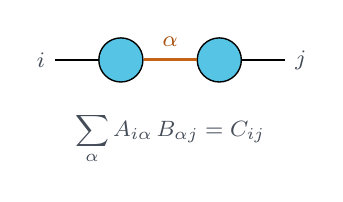
\begin{tikzpicture}[
    W/.style={circle, draw=black, fill=tnbulk, line width=0.5pt,
              minimum size=5.6mm, inner sep=0pt},
    leg/.style={draw=black, line width=0.5pt},
    lab/.style={font=\footnotesize, color=ink!85}]
  \node[W] (A) at (0,0)    {};
  \node[W] (B) at (1.25,0) {};
  \draw[leg] (A.west) -- ++(-0.55,0) node[lab,left]  {$i$};
  \draw[leg, tnbnd, line width=1.1pt] (A.east) -- (B.west)
        node[midway, above=1pt, lab, color=tnbnd!85!black] {$\alpha$};
  \draw[leg] (B.east) -- ++( 0.55,0) node[lab,right] {$j$};
  \node[lab, anchor=north] at (0.625,-0.55)
    {$\displaystyle\sum_\alpha A_{i\alpha}\,B_{\alpha j} = C_{ij}$};
\end{tikzpicture}
\end{document}
